% Chapter 1

\chapter*{Introduction} % Chapter title

\label{ch:introduction} % For referencing the chapter elsewhere, use \autoref{ch:introduction} 

%----------------------------------------------------------------------------------------

\minitoc

\section*{Nuclear Energy in France}

In 2020, France had a total of 136.2~GW of installed electrical power with a total production over the year of 500.1~TWh, 67.1\% of which coming from nuclear reactors (Figure \ref{fig:france_energy_mix}). Actually, nuclear energy plays a pivotal role in France's electrical mix since the 1950's and is promoted as a mean to reduce the global carbon dioxyde emissions of the country's energy production. The french government currently plans to build a total of six new nuclear reactors before 2050.

\begin{figure}[!h]
\centering
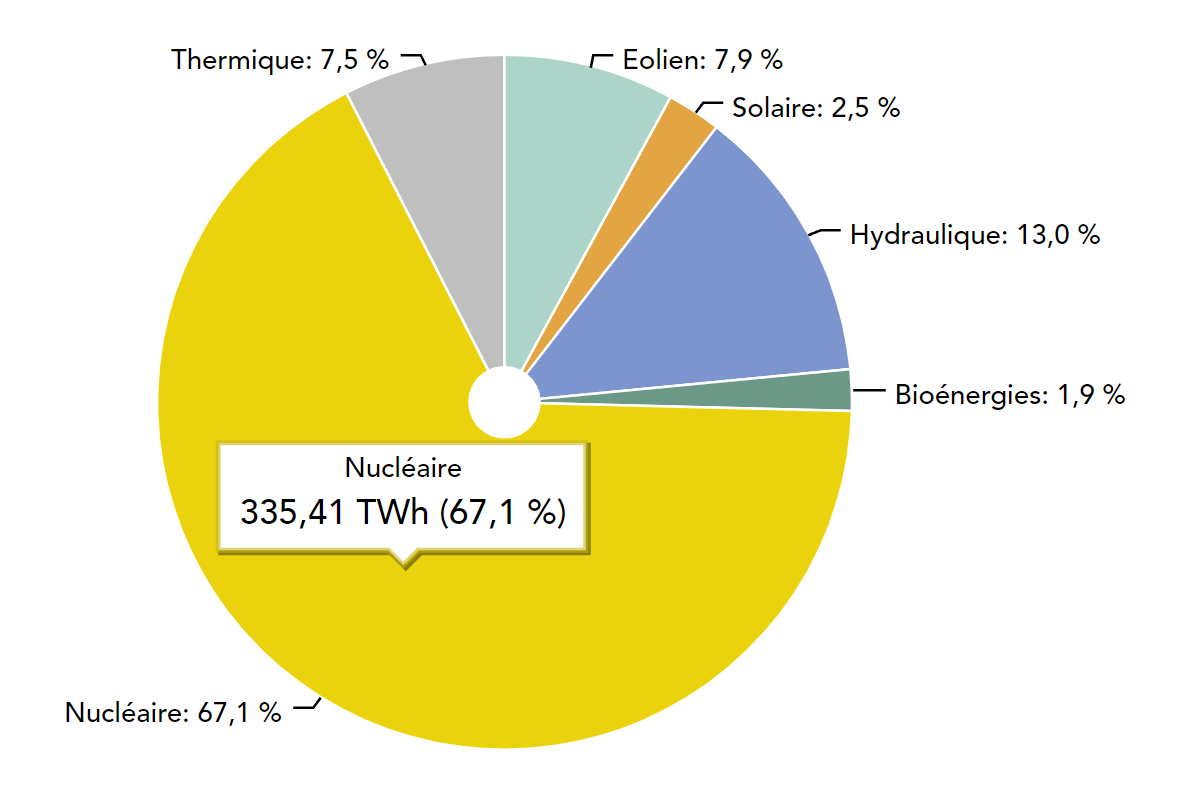
\includegraphics[width=0.6\linewidth]{img/intro/energy_mix.PNG}
\caption{Shared parts of energy production in France. \cite{rte_website} }
\label{fig:france_energy_mix}
\end{figure}

\npar

France accounts for a total of 56 nuclear power plants in 2020, all being Pressurized Water Reactors (PWR). They are dispatched over 19 different geographic locations and split in three electrical power series:

\begin{itemize}
\item 900~MW series (32 plants), launched between 1978 and 1988 (total installed power of 28.8~GW) ;
\item 1300~MW series (20 plants), launched between 1985 and 1994 (total installed power of 26.3~GW) ;
\item N4 series (1450~MW, 4 plants), launched between 2000 and 202 (total installed powed of 6~MW) being the most recent french PWR.
\end{itemize}


%%%%FIGURE OF NUCLEAR POWER PLANTS MAP



\section*{Physical and Technological Background}

\subsection*{Nuclear Energy}

\subsubsection*{Nuclear Fission}

On earth exists only one isotope that is called "fissile" : uranium 235 (noted $^{235}U$). Under certain physical conditions, $^{235}U$ collision with a neutron results in its break-up in two lighter atoms while releasing a total of two to three neutrons and an energy of the order of 200~MeV ($\approx 3.2 \times 10^{-11}$\ J). This amount of energy results from the mass difference between the $^{235}U$ and the products of the fission (atoms and neutrons), which is transferred as kinetic energy to the latter (Figure \ref{fig:fission}).



\begin{figure}[!h]
\centering
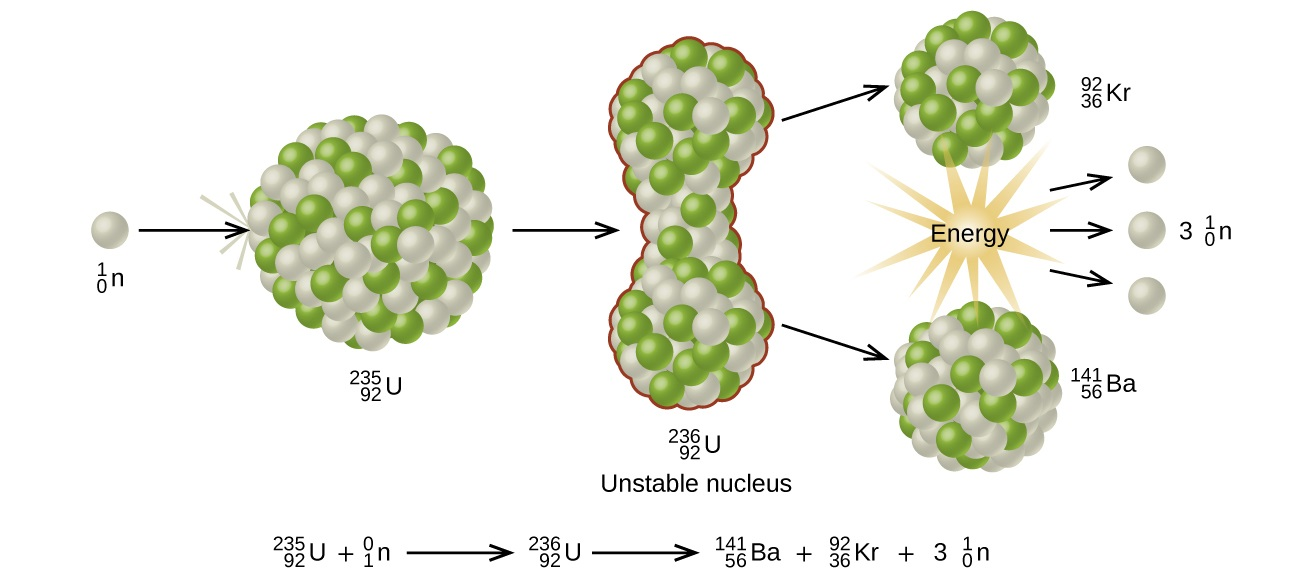
\includegraphics[width=0.6\linewidth]{img/intro/fission.jpg}
\caption{Sketch of the nuclear fission process. \cite{chem_libretext }}
\label{fig:fission}
\end{figure}


$^{235}U$ used in PWR is an isotope of uranium and accounts for only 0.7\% of the common uranium found in nature, most of which being uranium 238 ($^{238}U$) that is not fissile. For nuclear power production, common uranium must be enriched in $^{238}U$ up to 3\% to 5\%.

\subsubsection*{Nuclear Chain Reaction and Energy Production}


Fission presents particular interest for energy production due to its capacity to create a "nuclear chain reaction". Indeed, as multiple neutrons are expelled after the nuclear fission (Figure \ref{fig:fission}), each of them can potentially become a trigger for a new fission of a nearby $^{235}U$ atom. Since each fission releases more neutrons than required for its own triggering, this results in an exponentially increasing number of fission called a nuclear chain reaction.

\npar

However, neutrons actually released by the fission can't directly trigger a new one. They are emitted with a kinetic energy of approximately 2~MeV at which the probability of impacting an other $^{235}U$ is too low to start the nuclear chain reaction. Therefore, a so-called "moderator" is needed to slow down the neutrons through collisions with other atoms. Then the fission reactions lead the nuclear fuel to heat up rapidly and thus needs to be cooled to evacuate the produced energy. Using a fluid, it must both act as a coolant and allow the nuclear chain reaction to continue (moderator role). In french PWR, this is achieved using water as cooling fluid which also moderates the neutrons going through it.

\begin{note*}{}
Other nuclear reactor technologies exist with different fluid such as gas-cooled reactor using graphite as moderator material and carbon dioxyde as coolant.
\end{note*}

\npar

Following the heat exchange between the nuclear fuel and the water, the thermal energy stored in it can be used in a thermodynamic cycle (\eg Hirne cycle) to produce electrical power.



\subsection*{PWR Structure and Operation}

Pressurized Water Reactors are the only type of nuclear power plants operated in France for electricity production. A simplified sketch of a PWR is presented on Figure \ref{fig:pwr_sketch}.

\begin{figure}[!h]
\centering
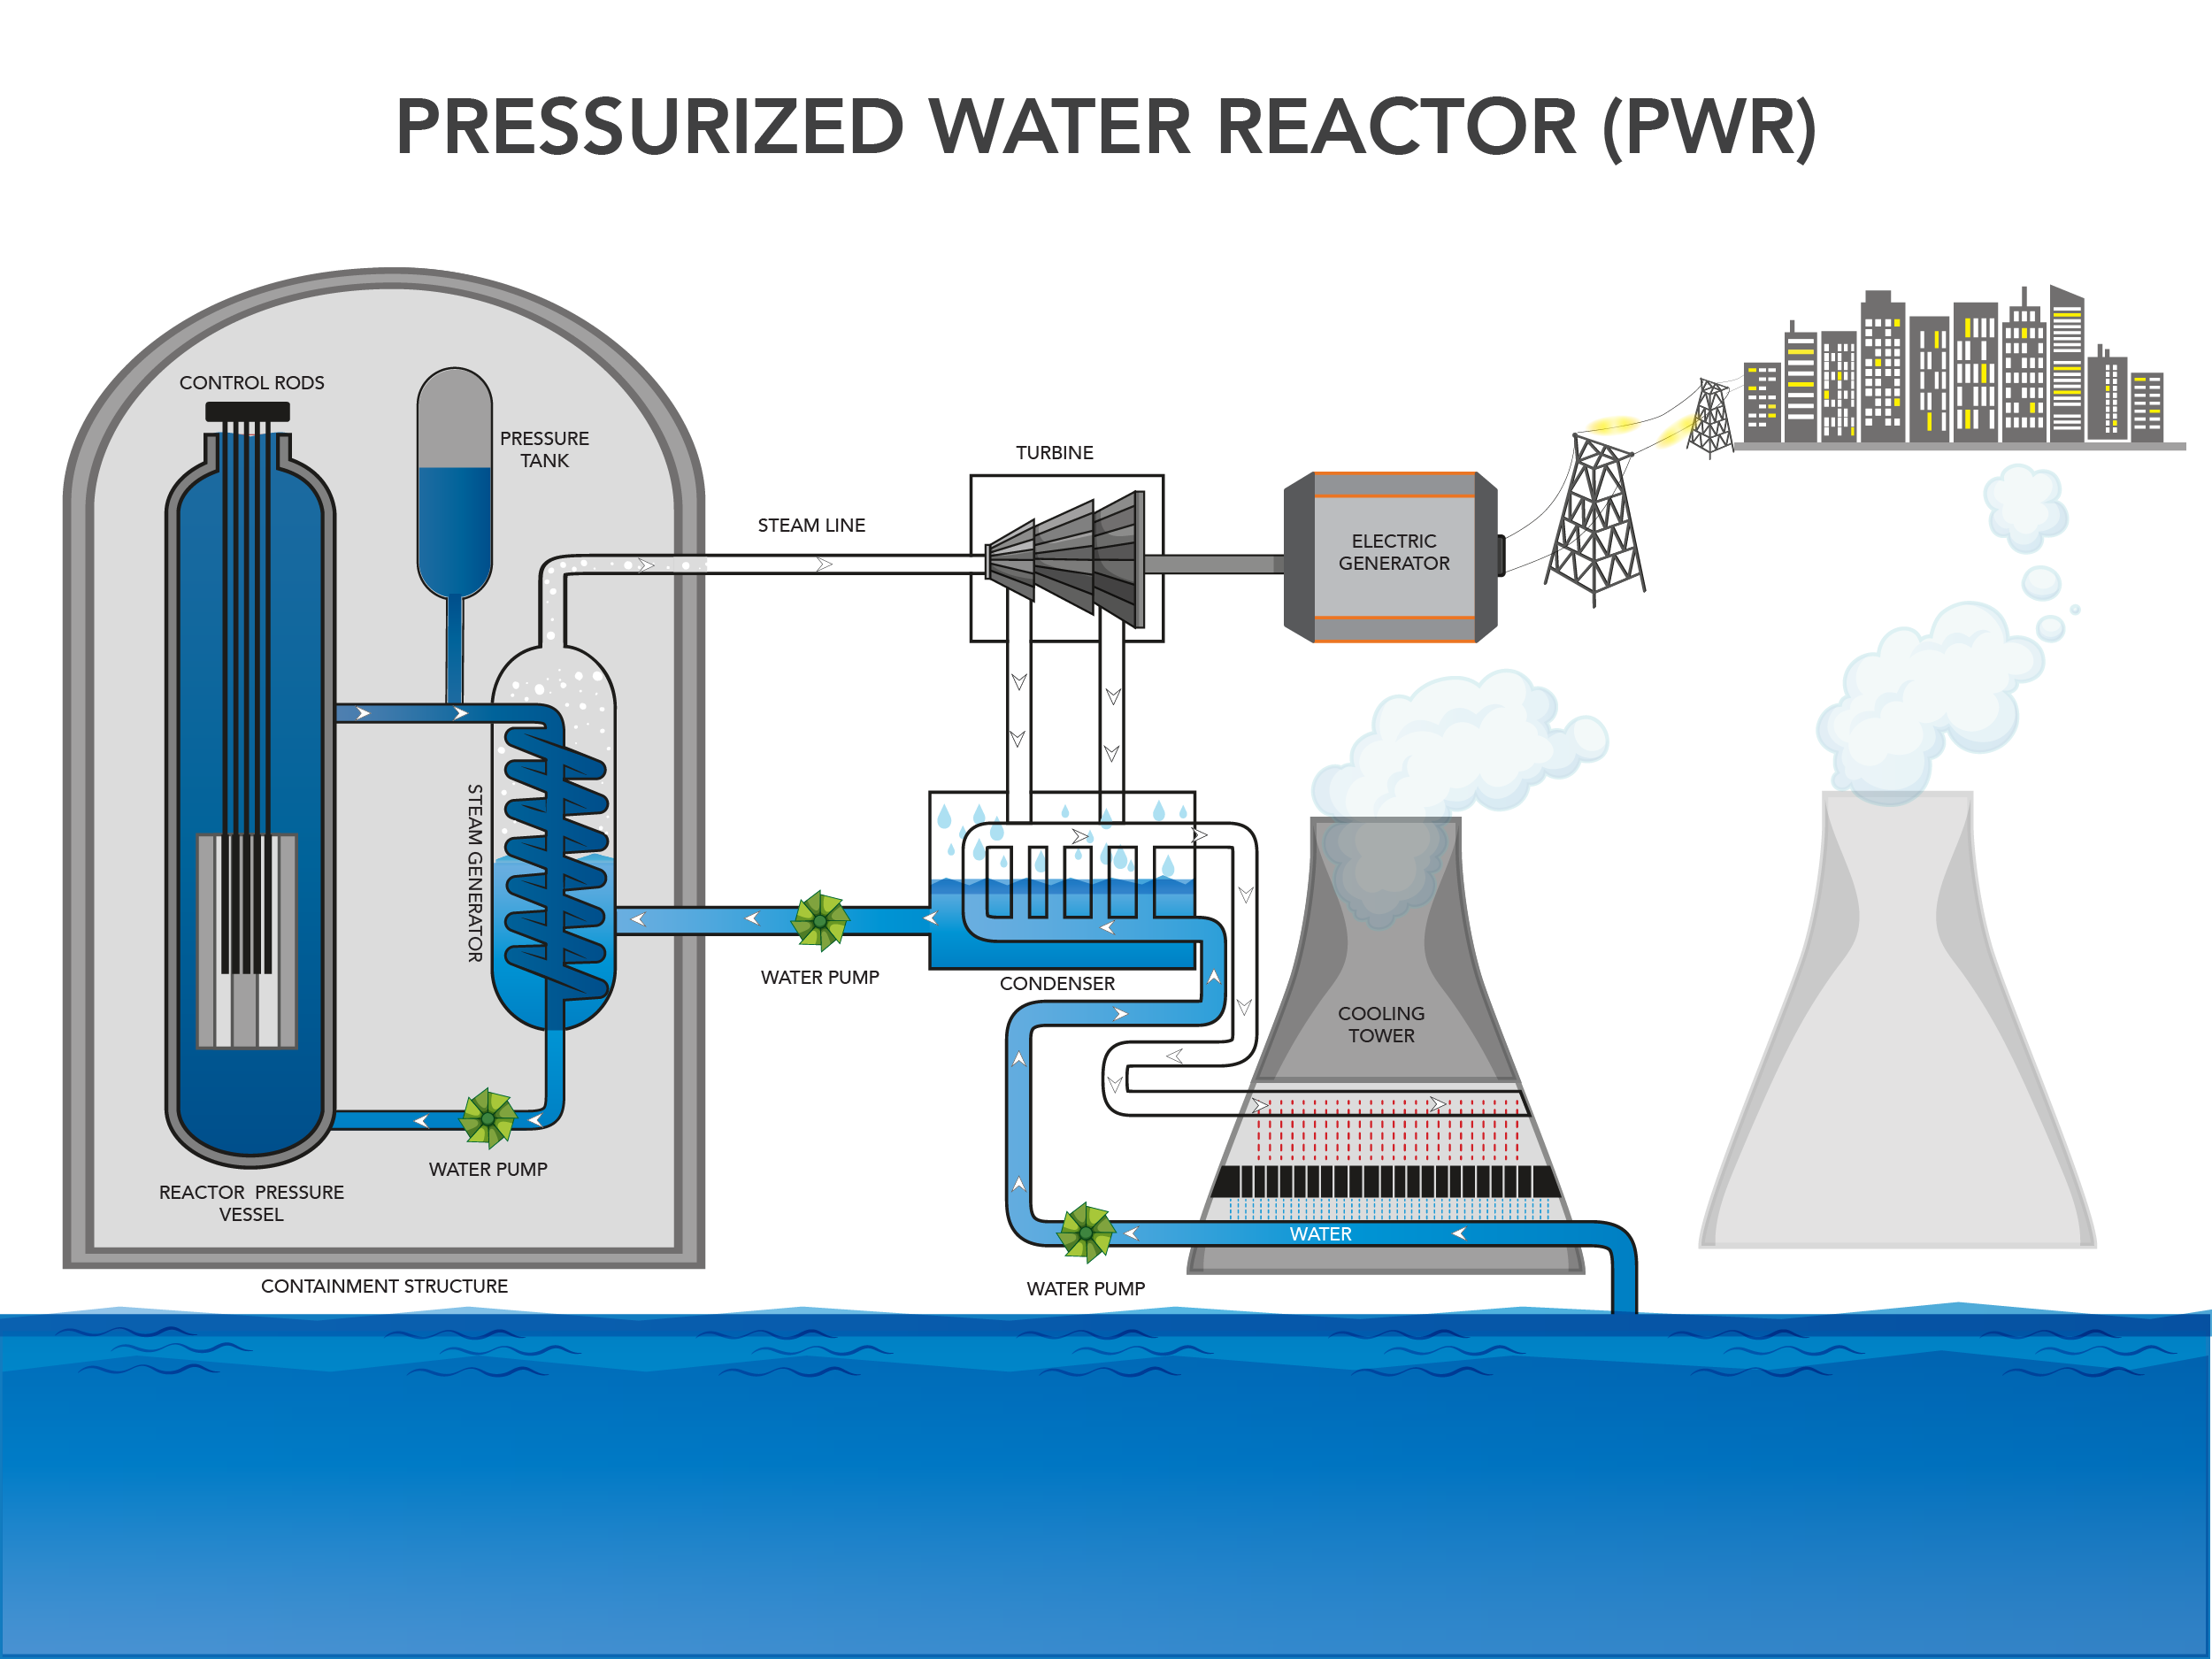
\includegraphics[width=0.7\linewidth]{img/intro/pwr_sketch.png}
\caption{Sketch of a Pressurized Water Reactor \cite{office_nuclear_energy}}
\label{fig:pwr_sketch}
\end{figure}



\subsubsection{Primary Circuit}

The primary circuit aims to collect the thermal energy expelled by the fission reactions within the nuclear fuel rods. The water flowing through the core gathers this energy and transfer it towards the vapor generator, while ensuring a moderating effect to maintain the nuclear chain reaction in the fuel. The primary circuit is fully closed and operates at a pressure close to 155\ bar, a temperature of $300\degC$ and mass flow rates between $3000$ and $5000 \debm$ (approximately 20 tons per second).  


To write :

\begin{itemize}
\item nuclear in france
\item progressive zoom toward the primary circuit and nuclear fuel assembly
\item heat transfer and boiling
\item CHF issue
\item Modeling, component approach, THYC
\item New approaches, CFD, objective of the thesis
\end{itemize}
